% !TeX spellcheck = fr_FR
%\addcontentsline{toc}{chapter}{Annexes} % Adding toc entry
%%% COMMENT THESES LINES IF YOU DO NOT USE DEDICATED TOC FOR ANNEXES
%\stopcontents[default]
%\resumecontents[annexes]
%%% /COMMENT THESES LINES IF YOU DO NOT USE DEDICATED TOC FOR ANNEXES
%\chapter*{Annexes}

% \begin{center}
% \textit{Imprimer idéalement cette page sur une page de couleur.}
% \textit{Chaque annexe doit commencer sur une nouvelle page et doit être numérotée : Annexe 1 puis Annexe 2, etc.}
% \end{center}


\chapter*{Annexe 1: Tableau des champs de l'en-tête de fichier LAS}
\addcontentsline{toc}{chapter}{Annexe 1: Tableau des champs de l'en-tête de fichier LAS}
\begin{table}[htpb!]
\centering
\begin{tabular}{|l|l|c|c|}
\hline
\multicolumn{1}{|c|}{\textbf{Champ}} & \multicolumn{1}{c|}{\textbf{Type de donnée}} & \textbf{Taille (Octets)} & \textbf{Requis} \\ \hline
File Signature (“LASF”)              & char{[}4{]}              & 4     & * \\ \hline
File Source ID                       & unsigned short           & 2     & * \\ \hline
Global Encoding                      & unsigned short           & 2     &   \\ \hline
Project ID - GUID data 1             & unsigned long            & 4     &   \\ \hline
Project ID - GUID data 2             & unsigned short           & 2     &   \\ \hline
Project ID - GUID data 3             & unsigned short           & 2     &   \\ \hline
Project ID - GUID data 4             & unsigned char{[}8{]}     & 8     &   \\ \hline
Version Major                        & unsigned char            & 1     & * \\ \hline
Version Minor                        & unsigned char            & 1     & * \\ \hline
System Identifier                    & char{[}32{]}             & 32    & * \\ \hline
Generating Software                  & char{[}32{]}             & 32    & * \\ \hline
File Creation Day of Year            & unsigned short           & 2     &   \\ \hline
File Creation Year                   & unsigned short           & 2     &   \\ \hline
Header Size                          & unsigned short           & 2     & * \\ \hline
Offset to point data                 & unsigned long            & 4     & * \\ \hline
Number of Variable Length Records    & unsigned long            & 4     & * \\ \hline
Point Data Format ID (0-99 for spec) & unsigned char            & 1     & * \\ \hline
Point Data Record Length             & unsigned short           & 2     & * \\ \hline
Number of point records              & unsigned long            & 4     & * \\ \hline
Number of points by return           & unsigned long{[}5{]}     & 20    & * \\ \hline
X scale factor                       & double                   & 8     & * \\ \hline
Y scale factor                       & double                   & 8     & * \\ \hline
Z scale factor                       & double                   & 8     & * \\ \hline
X offset                             & double                   & 8     & * \\ \hline
Y offset                             & double                   & 8     & * \\ \hline
Z offset                             & double                   & 8     & * \\ \hline
Max X                                & double                   & 8     & * \\ \hline
Min X                                & double                   & 8     & * \\ \hline
Max Y                                & double                   & 8     & * \\ \hline
Min Y                                & double                   & 8     & * \\ \hline
Max Z                                & double                   & 8     & * \\ \hline
Min Z                                & double                   & 8     & * \\ \hline
\end{tabular}
\caption[Champs de l'en-tête d'un fichier LAS]{Champs de l'en-tête d'un fichier LAS}
\label{tab:las_header}
\end{table}

\chapter*{Annexe 2 : Implémentation de la recherche de site candidat pour la fusion}
\addcontentsline{toc}{chapter}{Annexe 2 : Implémentation de la recherche de site candidat pour la fusion}

\begin{lstlisting}[language=Rust, style=boxed]
loop {
    let candidate_right = Mesh::get_side_candidate(
        other,
        r_bs,
        &self.vertices[l_bs]);
    let candidate_left = Mesh::get_side_candidate(
        self,
        l_bs,
        &other.vertices[r_bs]);
    let candidates = (candidate_left, candidate_right);
    match candidates {
        (Some(l), Some(r)) => {
            // Check that one of these does not contain the other one
            let left_candidate_inside = self
					.vertices[l]
					.inside_circum_circle((
					&self.vertices[l_bs],
					&other.vertices[r_bs],
					&other.vertices[r],
					));
            let right_candidate_inside = other
                    .vertices[r]
                    .inside_circum_circle((
                        &self.vertices[l],
                        &self.vertices[l_bs],
                        &other.vertices[r_bs],
                    ));
            match (left_candidate_inside, right_candidate_inside) {
                // If both are contained in each other
                // it is a degenerate case and there
                // is no possible outcome
                // to have a good Delaunay triangulation
                (false, false) => 
                        return Err(
                        "Edge case found about 4 co-circular points"
                        ),
                (true, false) => {
                    edges.push(l);
                    edges.push(r_bs);
                    l_bs = l;
                }
                (false, true) => {
                    edges.push(l_bs);
                    edges.push(r);
                    r_bs = r;
                }
                _ => break,
            }
        }
        (Some(l), None) => {
            // Connect it to the lr base,
            // push the new triangle and move the l_bs reference
            edges.push(l);
            edges.push(r_bs);
            l_bs = l;
        }
        (None, Some(r)) => {
            // Connect it to the lr base, 
            // push the new triangle and move the r_bs reference
            edges.push(l_bs);
            edges.push(r);
            r_bs = r;
        }
        _ => {
            // The merging is done if it doesn't exists anymore candidates
            break;
        }
    }
}
\end{lstlisting}

% \chapter*{Annexe 2}
% \addcontentsline{toc}{chapter}{Annexe 2}
% 
% 
\chapter*{Annexe 3 : Implémentation du voisinage d'un maillage}
\addcontentsline{toc}{chapter}{Annexe 3 : Implémentation du voisinage d'un maillage}

\begin{lstlisting}[language=Rust, style=boxed]
pub fn neighbourhood(&mut self) -> Option<Vec<HashSet<usize>>> {
        if self.neighbourhood.is_some() {
            return self.neighbourhood.clone();
        }
        let mut dict: Vec<HashSet<usize>> = 
            vec![HashSet::new(); self.vertices.len()];

        // Iterating over all triangles in the mesh
        self.faces
            .iter()
            .enumerate()
            .step_by(3)
            .for_each(|(i, _): (usize, &usize)| {
                // Adding the neibours of the first vertex
                dict[self.faces[i]].insert(self.faces[i + 1]);
                dict[self.faces[i]].insert(self.faces[i + 2]);

                // Adding the neibours of the second vertex
                dict[self.faces[i + 1]].insert(self.faces[i]);
                dict[self.faces[i + 1]].insert(self.faces[i + 2]);

                // Adding the neibours of the third vertex
                dict[self.faces[i + 2]].insert(self.faces[i]);
                dict[self.faces[i + 2]].insert(self.faces[i + 1]);
            });

        self.neighbourhood = Some(dict.clone());
        Some(dict)
}
\end{lstlisting}

\chapter*{Annexe 4 : Configuration de l'ordinateur sur lequel les test ont été
effectués}
\addcontentsline{toc}{chapter}{Annexe 4 : Configuration de l'ordinateur de tests}
\begin{figure}[htbp!]
    \centering
    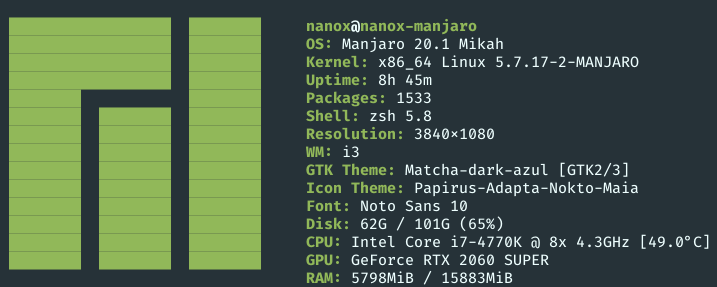
\includegraphics[width=0.8\linewidth]{figures/configs.png}
    \caption{Configuration de l'ordinateur de tests. Source : réalisé par Jérôme Chételat}
	\label{fig:computer_configuration}
\end{figure}

%%% COMMENT THESES LINES IF YOU DO NOT USE DEDICATED TOC FOR ANNEXES
\stopcontents[annexes]
\resumecontents[default]
%%% /COMMENT THESES LINES IF YOU DO NOT USE DEDICATED TOC FOR ANNEXES
